\documentclass{standalone}
\usepackage{tikz}
\usetikzlibrary{shapes.geometric, arrows, positioning}

\tikzset{
  flowblock/.style={
    rectangle,
    rounded corners,
    minimum width=3cm,
    minimum height=1cm,
    align = center,
    draw=black,
    line width = 1pt,
  },
  arrow/.style={
    line width = 1.5pt,
    ->,
    > = stealth,
    draw=black!70,
    },
  bentarrow/.style={
    line width = 1.5pt,
    ->,
    > = stealth,
    draw=black,
    bend left=20,
    },
}

\begin{document}
  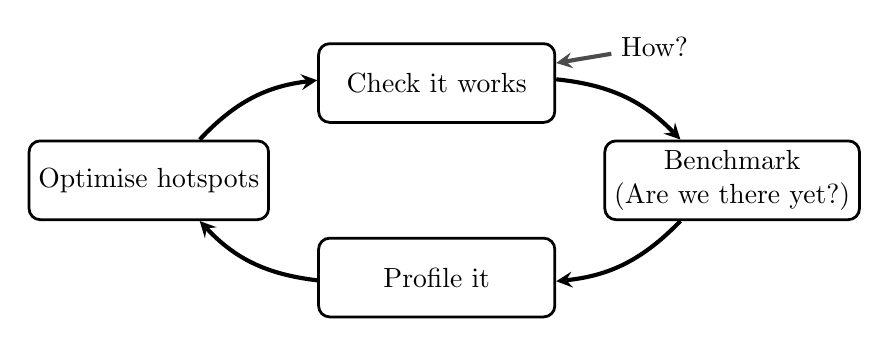
\begin{tikzpicture}
    \node (1) [flowblock,] {Check it works};
    \node (2) [flowblock, below right = 0.2cm and 0.6cm of 1] {Benchmark\\(Are we there yet?)};
    \node (3) [flowblock, below left = 0.2cm and 0.6cm of 2] {Profile it};
    \node (4) [flowblock, below left = 0.2cm and 0.6cm of 1] {Optimise hotspots};
    \node (5) [above right = -0.3cm and 0.7cm of 1] {How?};
    \draw [bentarrow] (1) to (2);
    \draw [bentarrow] (2) to (3);
    \draw [bentarrow] (3) to (4);
    \draw [bentarrow] (4) to (1);
    \draw [arrow] (5) -> (1);
  \end{tikzpicture}
\end{document}
